% THIS IS AN EXAMPLE DOCUMENT FOR VLDB 2012
% based on ACM SIGPROC-SP.TEX VERSION 2.7
% Modified by  Gerald Weber <gerald@cs.auckland.ac.nz>
% Removed the requirement to include *bbl file in here. (AhmetSacan, Sep2012)
% Fixed the equation on page 3 to prevent line overflow. (AhmetSacan, Sep2012)

\documentclass{vldb}
\usepackage{listings}
\usepackage{graphicx}
\usepackage[lined,commentsnumbered,linesnumbered]{algorithm2e}
\usepackage{subcaption}
\usepackage[labelfont=bf]{caption}
\usepackage{balance}  % for  \balance command ON LAST PAGE  (only there!)

\usepackage[usenames,dvipsnames]{xcolor}

\usepackage{amsfonts}
\usepackage{amssymb}
\usepackage{amsmath}
\usepackage{latexsym}
\usepackage{verbatim}
\usepackage{url}
\usepackage{color}
\usepackage{array}
\usepackage{textcomp}
\usepackage{paralist}
\usepackage{comment}
%\usepackage{times}
\usepackage{pifont,array,amsmath,multirow,latexsym,tabularx,amssymb}

\usepackage{hyperref}
\usepackage{url}
\usepackage{xspace}

\usepackage[usenames,dvipsnames]{xcolor}

\usepackage{times}
%\usepackage{MinionPro}

\usepackage{alltt}


%\usepackage{fullpage}
\usepackage{graphicx}
\usepackage{xspace}
\usepackage{amsmath}
\usepackage{amssymb}
\usepackage{color}

\usepackage{float}
\usepackage{listings}


\newcommand*{\bmfontA}{\fontfamily{fvs}\selectfont}
%\newcommand*{\bmfontAA}{\fontfamily{pzc}\selectfont}
%\newcommand*{\bmfontAAA}{\fontfamily{lmr}\selectfont}
\newcommand*{\bmfontB}{\fontfamily{fi4}\selectfont}
\newcommand*{\bmfontC}{\fontfamily{lmss}\selectfont}
\newcommand*{\bmfontD}{\fontfamily{put}\selectfont}
\newcommand*{\bmfontE}{\fontfamily{ppl}\selectfont}
\newcommand*{\bmfontF}{\fontfamily{cmr}\selectfont}
\DeclareTextFontCommand{\bmfont}{\bmfontB}
\DeclareTextFontCommand{\bmfontt}{\bmfontA}
\DeclareTextFontCommand{\bmfonttt}{\bmfontC}
\DeclareTextFontCommand{\bmfontttt}{\bmfontD}
\DeclareTextFontCommand{\bmfonttttt}{\bmfontE}
\DeclareTextFontCommand{\bmfontttttt}{\bmfontF}
\DeclareTextFontCommand{\bmfonttttttt}{\bmfontG}

\newcommand{\estvar}[0]{var}
\newcommand{\system}[0]{\bmfont{\small VProfiler}}



\newcommand{\tofix}[1]{\textcolor{red}{#1}}
\newcommand{\rev}[1]{\textcolor{black}{#1}}
\newcommand{\cancut}[1]{\textcolor{green}{#1}}
\newcommand{\tempcut}[1]{}

\newcommand{\barzan}[1]{\textcolor{magenta}{BM: #1}}
%\newcommand{\barzan}[1]{}


\begin{document}

% ****************** TITLE ****************************************

\title{Identifying the Major Sources of Variance in Transaction Latencies:
Towards More Predictable Databases}

% possible, but not really needed or used for PVLDB:
%\subtitle{[Extended Abstract]
%\titlenote{A full version of this paper is available as\textit{Author's Guide to Preparing ACM SIG Proceedings Using \LaTeX$2_\epsilon$\ and BibTeX} at \texttt{www.acm.org/eaddress.htm}}}

% ****************** AUTHORS **************************************

% You need the command \numberofauthors to handle the 'placement
% and alignment' of the authors beneath the title.
%
% For aesthetic reasons, we recommend 'three authors at a time'
% i.e. three 'name/affiliation blocks' be placed beneath the title.
%
% NOTE: You are NOT restricted in how many 'rows' of
% "name/affiliations" may appear. We just ask that you restrict
% the number of 'columns' to three.
%
% Because of the available 'opening page real-estate'
% we ask you to refrain from putting more than six authors
% (two rows with three columns) beneath the article title.
% More than six makes the first-page appear very cluttered indeed.
%
% Use the \alignauthor commands to handle the names
% and affiliations for an 'aesthetic maximum' of six authors.
% Add names, affiliations, addresses for
% the seventh etc. author(s) as the argument for the
% \additionalauthors command.
% These 'additional authors' will be output/set for you
% without further effort on your part as the last section in
% the body of your article BEFORE References or any Appendices.

\numberofauthors{2} %  in this sample file, there are a *total*
% of EIGHT authors. SIX appear on the 'first-page' (for formatting
% reasons) and the remaining two appear in the \additionalauthors section.

\author{
% You can go ahead and credit any number of authors here,
% e.g. one 'row of three' or two rows (consisting of one row of three
% and a second row of one, two or three).
%
% The command \alignauthor (no curly braces needed) should
% precede each author name, affiliation/snail-mail address and
% e-mail address. Additionally, tag each line of
% affiliation/address with \affaddr, and tag the
% e-mail address with \email.
%
\alignauthor
Jiamin Huang\\
       \email{jiamin@umich.edu}
\alignauthor
Barzan Mozafari\\
       \email{mozafari@umich.edu}
}

\maketitle

%!TEX root = predictability.tex

\begin{abstract}
Transaction processing is an important part of modern database management
systems(DBMSs), so a lot of work has been done to improve the performance of
it. However, few people pay attention to the predictability of performance,
which is fundamental to many application of database systems such as
in-cloud database services that provide performance guarantee. The service
providers will not be able to provide such kind of guarantees unless their
services are based on database systems with predictable performance.

In this paper, we show that variance of transaction latency is a very
severe problem in traditional database systems like MySQL. We propose a
profiling framework called VProfiler that uses the source code of a database
system to identify the main sources of variance in transaction latency. This
framework works by breaking down the variance of latency into variances and
covariances of the execution time of the functions in the source code, which is
the best source of information about the actual cause of variance. Using MySQL
as an example, we show its main sources of variance found using our profiling
framework, and propose two methods to reduce the variance of latency after
close investigation of these sources. Experiment results show that these
two methods, when combined, achieve a 42.3\% reduction in 99th percentile.
Besides these methods, we also demonstrate how using faster storage devices and
tuning the configuration of MySQL can further improve its performance
predictability.
\end{abstract}



%!TEX root = predictability.tex

\section{Introduction}
\label{sec:intro}

Transactional databases are a key component of almost every enterprise software, where 
mission-critical applications rely on the underlying DBMS to store and manipulate data efficiently and reliably. 
Consequently, a significant portion of database research on transactions has focused on reducing latency and 
increasing  throughput, e.g.,  through
 concurrency control and recovery protocols, query optimization techniques, indexing schemes, 
 caching policies, \tofix{and many other sophisticated ideas.} 
These strategies, however, have been mostly evaluated  in terms of
 their effect on the \emph{average performance} of a transactional database, such as its throughput 
 or mean latency in executing transactions. 
 In other words, the focus has often been on running more and/or faster transactions \emph{overall}.
The effect of these strategies on the spread of the latency distribution has largely remained unvetted.
\tofix{Have our traditional database design principles sacrificed the tail latencies for the sake of improving average performance
of transactions? 
Do our existing databases exhibit a notable latency variance in practice?
If so, how much of this variance is due to 
our database implementation and how much of it is due to the 
the variations in the user's queries themselves?
How can we measure the contribution of each component/algorithm 
of our database to 
 the overall latency variance?
And most importantly,  do we need to compromise on the mean latency to reduce its variance or $99\%$ quantile, and if so, how?}

%ta inja 

We believe that it is critical and particularly timely to ask these questions. 
First, the past four decades of research on transactions has matured to a point where  
microsecond latencies and hundreds of thousands of concurrent transactions are now 
achievable \cite{??}.\tempcut{\footnote{Human-triggered transactions are bound by human population, and hence
are unlikely to grow rapidly in the foreseeable future; Amazon's ten million transactions on New Year's Eve 
translates to $7$K transactions per second. 
Applications that require higher throughputs are often triggered by machine-generated events    
and require much simpler semantics 
(e.g., sensor readings or high-frequency 
trading are often single-row transactions).}}
Second, database vendors are facing an increasing number of business-oriented clients and applications 
that demand
quality of service guarantees (QoS).\footnote{Based on oral communications with the chief architects, researchers and engineers at 
Teradata, HP Vertica, and Microsoft.} 
Moreover, with the increasing market-share of database-as-a-service  (DBaaS) offerings,
cloud providers and users rely on service level agreements (SLAs) for pricing and provisioning, respectively.
Finally, as they deliver 
a wide range of complex features to a wide range of applications,
DBMSs have (understandably) become one of the most complex breed of software systems \tofix{themselves}.
Thus, predicting query latencies in a database has  been reportedly one of the most 
challenging tasks~\cite{??}.
Understanding the major sources of variance in the execution time of transactions might provide 
invaluable insight towards designing a new generation of database systems that can deliver
competitive performance but be much more predictable.\footnote{While achieving
predictable performance is also desirable for analytical workloads, we leave this to future work
and only focus on transactional 
workloads in this paper.} 
The benefits of a predictable database will be many, e.g., automatic provisioning tools, 
more accurate cost estimates (and hence, better query scheduling and planning decisions), 
and more reliable 
query progress estimators. Identifying the major sources of variance 
% ta inja

Database Management Systems have become an essential part of almost every
large software system anyone can find today. Transaction processing is one of
the most important features provided by these database management systems,
which allows users to group a bunch of operations into one single logical
operation. A lot of work has been done on the performance of transaction
processing. Predictability of performance, which is just as important as
performance itself, remains neglected by researchers. An unpredictable database
management system is a potential cause of financial loss regardless of how good
the overall performance is. Due to the importance of predictability, many
enterprise companies are willing to sacrifice 10\% to 30\% of the overall
performance for a more predictable database. Predictability of performance is
an essential requirement for cloud-based offerings. For example, SQL Database
of Microsoft Azure, a relational database-as-a-service offering, provides
predictable performance guarantees in terms of Database Throughput Unit(DTU),
transaction rate and consistency of response time. On the other hand, the
Service Level Agreement(SLA) offered by Amazon's Relation Database Service(RDS)
is only in terms of Monthly Uptime Percentage, namely availability. For disks,
it offers performance guarantee only in terms of IOPS. No guarantees are
provided in terms of more interesting factors, such as transaction latency(
which is what the users really care about), and they will never exist unless
the provides base their database services on database management systems whose
performance is predictable.

We did experiments on MySQL to evaluate the predictability of their performance 
on transaction processing. MySQL is among the most widely used relational
database management systems(RDBMS) and most popular open-source RDBMS. It
provides not just one, but several storage engines for users to choose from,
among which Innodb is the default and most commonly used. Innodb is a storage
engine that provides standard ACID-compliant transaction features, along with
foreign key support. This paper is based on the Innodb engine.

We used Amazon EC2 m3.large instances with traditional HDDs in our experiments, 
and chose TPC-C as our benchmark. TPC-C is a famous Online Transaction
Processing(OLTP) benchmark. Queries in an OLTP system are mostly simple and
standardized with relatively small number of records returned. Unlike OLTP,
Online Analysis Processing(OLAP) systems are usually complex because of the
aggregations involved. Queries in OLTP systems are usually generated using
query templates. The following is a query template in the TPC-C Benchmark to
acquire data of an item from the database.

\begin{lstlisting}[
                language=SQL,
                showspaces=false,
                basicstyle=\ttfamily]
SELECT I_PRICE, I_NAME , I_DATA
FROM ITEM
WHERE I_ID = ACTUAL_ID
\end{lstlisting}

When this query is executed, \texttt{ACTUAL\_ID} would be replaced by an actual
value of an \texttt{I\_ID}, which could be different each time. Transactions in
OLTP systems are usually composed of a bunch of ordered query templates,
and can be categorized into different types according to the query templates
they consist of. TPC-C has five types of transactions: New Order, Payment,
Order Status, Delivery and Stock Level. The original TPC-C benchmark requires
45\% of New Order transactions, 43\% of Payment transactions, 4\% of Order
Status transactions, 4\% of Delivery transactions and 4\% of Stock Level
transactions. Transactions of the same type can also have different numbers of
queries(in a fixed range). These are all sources of variance in transaction
latency. Therefore, besides the original TPC-C benchmark, we also have
experiments that use only New Order transactions, and experiments that use New
Order transactions with fixed number of queries. We measure the average,
standard deviation and 99th percentile latency and use the ratio of standard
deviation to mean and the ratio of 99th percentile to mean to evaluate the
predictability of their performance.

\begin{figure}[h]
\centering
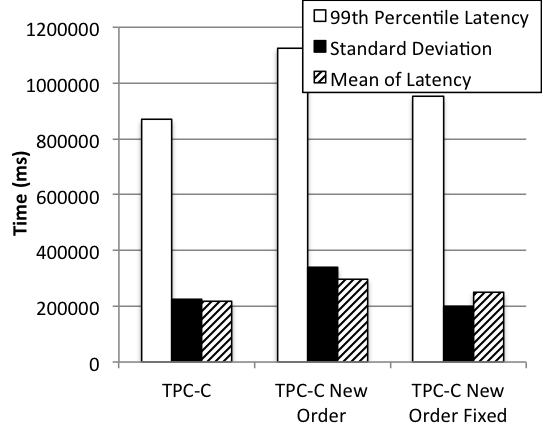
\includegraphics[scale=0.7]{plots/mysql-var}
\caption{99th percentile, standard deviation and average latency in MySQL}
\label{fig:mysql-var}
\end{figure}

\begin{figure}[h]
\centering
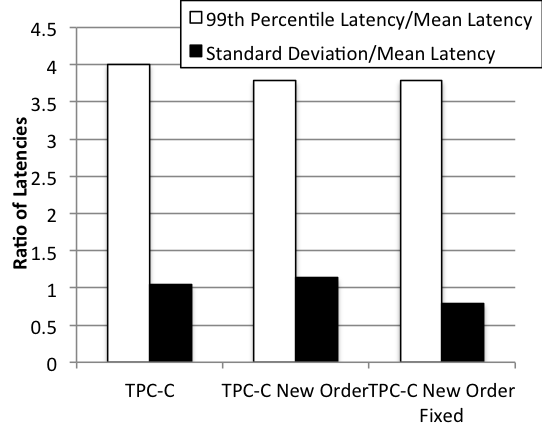
\includegraphics[scale=0.7]{plots/mysql-ratio}
\caption{99th percentile and standard deviation are several folds larger than
the average latency in MySQL}
\label{fig:mysql-ratio}
\end{figure}

As can be seen from figure \ref{fig:mysql-ratio}, the standard deviation of
transaction latencies is almost 3 times of the average latency. On the other 
hand, 99th percentile is a lot worse than standard deviation because no matter
which benchmark we use, the 99th percentile latency is an order of magnitude
larger then the average latency.



%!TEX root = predictability.tex

\section{Related Work}
Although relatively ignored compared to performance of transaction processing,
performance predictability has received some significant interest from the
research community. Studies have been done regarding query progression
indication and query performance prediction, architecture redesign and
predictability improvement.

\textbf{Query Progress Indication and Query Performance Prediction} There has
been significant work \cite{chaudhuri:can, chaudhuri:estimating, luo:toward, 
luo:increasing, luo:multi} about query progress indicators, which are used to
estimate the progress of long-running queries. In \cite{chaudhuri:can, 
chaudhuri:estimating, luo:toward, luo:increasing}, a set of techniques are
proposed to keep track of how much of a query has been completed and 
continuously estimate the remaining query execution time. These query progress
indicator, however, are single-query indicators, which means that they only
take the current workload and the estimated query into consideration, ignoring
the impact from all other currently running queries. A query indicator that
handles the performance impact of current queries is proposed in
\cite{luo:multi}, which even considers the influence of queries expected to
arrive in the future.

There are also work \cite{ahmad:interaction, duggan:performance, gupta:pqr,
ganapathi:predicting} about predicting the performance of queries that are not
yet executed. \cite{ahmad:interaction} proposes an approach to predict the
total execution time of a query workload consisting of different types of
queries that are executed concurrently. However, this paper focuses on
predicting the execution time of the whole workload, and does not address the
problem of predicting execution time of individual queries.

In \cite{ganapathi:predicting}, Archana \textit{et al.} propose a system that
uses machine learning techniques to predict multiple performance matrices of
database queries, including(but not limited to) records used, I/O operations
and most importantly, query latency. The drawback of this paper is that it
does not deal with concurrent workloads. Machine learning techniques are also
used in \cite{gupta:pqr}, which provides query latency prediction as time
ranges. \cite{duggan:performance} proposes a method for predicting the
performance of queries in concurrent OLAP workloads. Unlike the other papers,
it does not require semantic information, but rather uses a modeling approach
that depends on the analysis of query behavior in isolation, the interactions
of query in pairs and sampling techniques.

Query progress indication and query performance prediction are more about
predicting or estimating query latency. However, these paper make no attempt
to deal with the problem of performance unpredictability, that is, they do not
help to improve predictability matrices such as variance of latency, and 99th
percentile of latency.

\textbf{Architecture Redesign} People have thought of changing the design of
current database management systems to improve the predictability of 
performance. Surajit and Gerhard argue in \cite{chaudhuri:rethinking} that the 
performance of current database systems are unpredictable because they are
among the most complicated software systems ever built by humans and their
major components seldom get redesigned when new features are added, resulting
in a larger and larger and more and more complex code base that inherently
causes the unpredictability of the exact behavior and performance. They propose
building data management systems on RISC-style components, which are fairly
simple by themselves, but can be combined to create richer components. These
well-defined components with narrow functionality make it easier to predict and
tune the performance of the system. However, they discuss these problems from a
very high level perspective, and do not touch any implementation details. 
Neither do they present any design of a new data management system built upon a
set of RISC-style components.

Another paper that rethinks the design of database management system is
\cite{florescu:rethinking}. Daniela \textit{et al.} give a summary of the
requirements people have for database management systems, including 
performance, predictability, consistency, etc. However, due to the limitation
of resources, database developers have to sacrifice some of the requirements
for the others. Performance in terms of latency and throughput are usually
preferred while the others receive relatively less attention. The authors
point out that predictability is simply not taken into account when database 
developers design modern database management systems. The implementations of
the classic three-tier database architecture usually do not meet the
predictability requirement. Therefore they present a new three-layer
architecture in which consistency is maintained in the application layer and
the storage layer is only responsible for storing data. The new design makes it
possible to use a lot of cheap machines in the storage layer, unlike the
traditional three-tier architecture, where the database has to guarantee
consistency, and must be run on only a few expensive servers.

Again, this paper addresses the problem of predictability(and other properties)
from a very high level and gives no implementation details. Also, the new
architecture basically delegates part of the functionality of a database
to applications that uses databases, and therefore is incompatible with
existing systems. Finally, this new design makes applications more difficult to
build considering that they have to maintain data consistency themselves.

\textbf{Predictability Improvement} There has been work that proposes 
techniques to improve performance predictability. \cite{babcock:optimizer} 
deals with unpredictability in a more practical manner --- it approaches the
problem through the query optimizer. Traditionally, query optimizers use
execution time as the sole heuristic for deciding which query plan to select,
and ignore other important qualities, predictability being one of them. Brian
Babcock \textit{et al.}\ build a new optimizer that uses a probability
distribution over possible selectivity, which quantifies the estimation
uncertainty and allows the optimizer to select the most appropriate query plan
based on the pre-defined relatively importance of performance versus
predictability.





%!TEX root = predictability.tex

\section{Identifying the Main Sources\\ of Variance}
Database Management Systems are very complex systems, and there are many
possible sources of variance, such as I/O operations, locking, thread
scheduling, etc. There are tools to gather information about these events.
For example, using strace, you can collect data about every I/O operation
including size of data read or written, time of each I/O operation, etc.
However, such kind of information is not intuitive enough for explaining
the variance of latency even for the most skilled database administrators.
Moreover, these tools are usually related to the kernel, thus introducing
overhead such as context switching for each system call. This could be quite 
expensive and would also introduce noise into the latency data. These tools,
therefore, are not suitable for analyzing the source of variance. We tackle
this problem using a different approach.

\subsection{Variance Break Down}
The latency of a transaction is the time it takes to process a transaction, and
the processing of a transaction can be traced down to some high level function 
in the system's source code that is responsible for executing the queries. In
MySQL, this high level function is called \texttt{dispatch\_command}.
Therefore, the latency of a transaction is basically the execution time of this 
high level function during a transaction, and the variance of latency is the
variance of the execution time of this function in different transactions.

\begin{figure*}
\centering
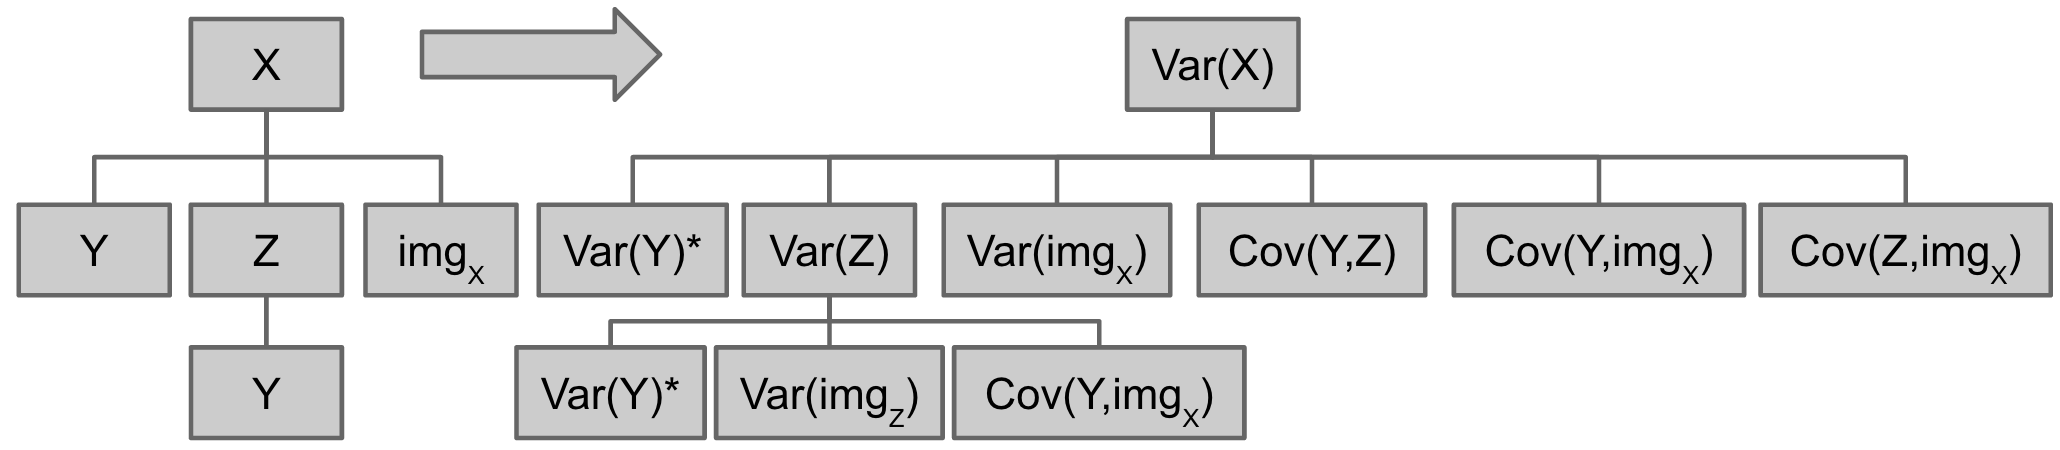
\includegraphics[scale=0.5]{plots/var_break_down}
\caption{A static call graph and its corresponding \textit{variance tree}}
\label{fig:var_break_down}
\end{figure*}

Most of the time, a function has to call other functions to accomplish its
job. A function's execution time is roughly the total execution time of all
the functions it calls. In this paper, we refer to the function that calls
other functions as the \textit{parent function}, and those being called as the
\textit{child functions} of it. For example, if function X calls function Y and
Z, then X would be the \textit{parent function} of Y and Z and they would
be the \textit{child functions} of X. Let $E(f)$ denote the execution time of
function f, we have
\begin{displaymath}
E(X) = E(Y) + E(Z)
\end{displaymath}

However, strictly speaking, this is incorrect because besides calling function
Y and Z, function X also has to execute some other basic statements, like
variable assignments, if statements, etc. The time spent on them, although
might be way smaller than the time spent on function Y and Z, must also be
considered. To model this, we can add an \textit{imaginary function} $img_X$
to the list of children of X. In this way, we can now say that function X does
nothing other than calling function Y, Z and $img_X$, and so
\begin{displaymath}
E(X) = E(Y) + E(Z)+ E(img_X)
\end{displaymath}

Let's say $E(X)$ has a large variance and we would like to know why. Since the
only thing X does is invoking function Y, Z and $img_X$, we know that one or
more of these functions are to blame for the variance. To find out the 
functions that cause $E(X)$ to have a large variance, we need to quantify
the contribution of each and every \textit{child function} of X.

Variance can be calculated in many ways, the following one being one of them:
\begin{equation}
Var(\sum_{i=1}^{n}X_i) = \sum_{i=1}^{n}Var(X_i) + 2\sum_{1\leq i}\sum_{\leq j \leq n}Cov(X_i, X_j)
\label{eq:var-break-down}
\end{equation}
Using this formula, we can easily break down the variance of $E(X)$ into the
variances and covariances of the execution time of function Y, Z and $img_X$,
in which the variances can be further broken down by applying the same formula.
For the rest of this paper, we use the term ``variance of a function'' as an
abbreviation for the variance of the execution time of a function, and the term
``covariance of two functions'' as the abbreviation for the covariance of two
functions' execution time for simplicity. Figure \ref{fig:var_break_down} shows
the result of breaking down the variance of X. The graph on the left is the
static call graph, which shows that function X calls functions Y, Z, and $img_X$.
The graph on the right shows that the variance of X can be broken down into
the variances of Y, Z, $img_X$, and the covariances of every two of them. It
also shows how the variance of Z can be further broken down. We call this graph
a \textit{variance tree}.

Variance break down is fairly easy to do with the source code. Given a 
function, we can inserted a small piece of code into the source code of this
function to retrieve the timestamp at the beginning and end of this function,
and then calculate its execution time using these two timestamps easily. 
Similarly, for each function call in this function, we retrieve the timestamp
before and after the function call and calculate the execution time 
accordingly.

Applying this technique on the functions in MySQL responsible for query
processing allows us to see each function's contribution to the overall
variance and locate those with significant contributions. Looking only at the
value of variance or covariance is not enough, though. An obvious example is
that function \texttt{dispatch\_command} contributes to 100\% of the variance
of latency, but it barely gives us any useful information about the cause of
the variance. This means that we also need to consider how useful a function is
in helping us find out the actual cause behind the high variance.

Another thing to notice is that, a function can be called in different places
in the source code, so there can be multiple nodes in the \textit{variance
tree} that represent the variance of the same function or the covariance of the
same functions, each with a possibly different value. For example, in figure
\ref{fig:var_break_down}, both function X and Z calls function Y, and so in the
\textit{variance tree}, there are two nodes that both represent the variance of
function Y(marked with asterisk). It is possible that to reduce the variance X,
we need to change the implementation of Y, which would affect the values of
both nodes. Therefore, we must consider them all together. We use the term
\textit{factor} to represent the variance of a function or the covariance of
two functions during the execution of a transaction. On the other hand, the
nodes in the \textit{variance tree} represents the variance of a function or
the covariance of two functions only during the execution of some particular
function. We call them the \textit{instances} of the \textit{factor}. Each
node in the \textit{variance} corresponds to an \textit{instance}. In figure
\ref{fig:var_break_down}, Var(Y) is a \textit{factor}, and the two nodes marked 
with asterisks in the \textit{variance tree} are \textit{instances} of
\textit{factor} Var(Y).

The goal of finding the main sources of variance in transaction latency
now turns into finding the \textit{factors} such that:

\begin{itemize}
    \item make significant contributions to the variance of transaction latency
    \item give us enough information about the cause of variance
\end{itemize}

\subsection{Factor Selection}
To select \textit{factors} that satisfy the two criteria mentioned above, we 
need to quantify them. The first one can be quantified by the value of variance 
or covariance. For the rest of this paper, we use the term 
\textit{contribution} to represent the value of variance of covariance. An
intuition to quantify the second criterion is that, the more specific a
function is about what it does, the more information it can
give us about the cause of its variance. Moreover, a \textit{child function} is
usually more specific about its job than its \textit{parent function}.

For example, a function A that writes several log records to the global log
buffer must first acquire the lock on the log buffer(function B), copy the
log data to the log buffer(function C), and finally release the
lock(function D). Let us say function A's variance is 30\% of the
variance of latency and function C's variance is 28\% of the variance
of latency. We would find function C more interesting than function A
because even though its variance is smaller than that of function A, it
has narrower functionality and is more specific. It's possible that a closer
look at this function can tell us that its variance is caused by the size of
log data being copied to the log buffer each time, and so a solution that
reduces log size variance could effectively reduce the overall variance.

Therefore, the ``specificness'' of a \textit{factor} is related to the
heights of the functions involved. Also, given a call graph, no matter how 
many different places a function occurs, all these nodes have the same 
height. We can use existing call graph generation tools likes CodeViz
\footnote{http://www.csn.ul.ie/\textasciitilde{}mel/projects/codeviz/} to
generate the call graph and pre-compute the height of any given function. Most
of the time, the smaller the height is, the more specific the function is about
what it does. With this intuition, we can define the ``specificness'' of a
\textit{factor} as a decreasing function of the heights of the functions
involved. In our experiments, we use the following function:
\begin{equation}
speci(N) = (height(call\_graph) - height(N))^3
\label{eq:speci}
\end{equation}
In this function, $height(call\_graph)$ is the height of the sub call graph
whose root is function \texttt{dispatch\_command}. $height(N)$ is the height of 
the function if $N$ represents the variance of function, and the larger height
if $N$ represents the covariance of two functions.

Now we can define the responsibility of a \textit{factor} to the overall
transaction latency as
\begin{equation}
resp(N) =  speci(N)\sum_{i}contri(N_i)
\label{eq:resp}
\end{equation}
where N is a \textit{factor} and $N_i$ are \textit{instances} of this
\textit{factor} in the \textit{variance tree}.

\begin{algorithm}[t]
    \SetAlgoLined
    \SetKwInOut{Input}{Inputs}
    \SetKwInOut{Output}{Output}
    \SetKwFunction{FactorOf}{factor\_of}
    \SetKwFunction{NewFactor}{new\_factor}
    \SetKwFunction{Speci}{speci}
    
    \Input{
        $t$, variance break-down tree,\\
        $k$: maximum number of functions to select,\\
        $d$: threshold for minimum contribution}
        
    \Output{
        $s^*$: top $k$ most responsible factors}
    \BlankLine
        
    $h \gets $ empty list\;
    \BlankLine    
    
    \ForEach{$ node~ N \in t$} {
        $N^* \gets \FactorOf{h, N}$\;
        \uIf{$N^* = NULL$} {
            $N^* \gets \NewFactor{}$\;
            $N^*.contri \gets 0$\;
            $h \gets h \cup N^*$\;
        }
        \uElse{
            $N^*.contri \gets N^*.contri + N.contri$\;
        }
    }
    \BlankLine    
    
    \ForEach{$N^* \in h$} {
        $N^*.resp = \texttt{speci}(N^*) \cdot N^*.contri$\;
    }
    \BlankLine
    
    Sort $h$ in descending order of $N^*.resp$\;
    \BlankLine
    
    $s^* \gets$ empty list\;
    \For{$ i \gets 1$ \KwTo $k$} {
        $N^* \gets h[i]$\;
        \uIf{$N^*.contri \geq d$} {
            $s^* \gets s^* \cup N^*$\;
        }
        \uElse{
            break\;
        }
    }
    
    \KwRet{$s^*$}\;
    
\caption{Factor Selection}
\label{alg:factor-selection}
\end{algorithm}

Given the \textit{variance tree}, we now propose an algorithm to select the top
k most responsible \textit{factors} from this tree for the variance of latency.
The pseudocode is shown in algorithm \ref{alg:factor-selection}. The basic
idea of this algorithm is very simple. We iterate over the \textit{variance 
tree}, and for each node, and check if the \textit{factor} of this node is 
already in list $h$. If not, we add the \textit{factor} to $h$. If the
\textit{factor} is already in $h$, we need to add the contribution of this
node(the value of variance of covaraince) to the contribution \textit{factor}
(line 1 to line 10). After we find all \textit{factors}, we calculate their
\textit{resp} values using equation \ref{eq:resp} (line 11 to 13). After that,
we sort the \textit{factors} in descending order of their \textit{resp} values,
and select the ones with a total contribution value greater than or equal to
threshold $d$ from the first $k$ elements of list $h$(line 14 to 23).

\subsection{VProfiler: A Variance Source Discovery Framework}

\begin{algorithm}[t]
    \SetAlgoLined
    \SetKwInOut{Input}{Inputs}
    \SetKwInOut{Output}{Output}
    \SetKwFunction{VarBreakDown}{var\_break\_down}
    \SetKwFunction{SetRoot}{set\_root}
    \SetKwFunction{AddChildren}{add\_children}
    \SetKwFunction{SelectFactors}{select\_factors}
    \SetKwFunction{NeedsBreakDown}{needs\_break\_down}
    \SetKwFunction{GetInstanceOf}{get\_instance\_of}
    \SetKwFunction{IsVariance}{is\_variance}
    \SetKwFunction{Clear}{clear}
    
    
    \Input{
        $v$: variance of function $dispatch\_command$,\\ 
        $k$: maximum number of functions to select,\\
        $d$: threshold for minimum contribution,\\
        $m$: threshold for minimum relatively contribution of children}
        
    \Output{
        $s^*$: top $k$ most responsible factors}
    \BlankLine
        
    $t \gets$ empty tree\;
    $t.\SetRoot{v}$\;
    $l \gets$ empty list\;
    $l \gets l \cup v$\;
    $e \gets true$\;
    \BlankLine
    
    \While{$e$} {
        \BlankLine
        
        \ForEach{$factor~ f \in l$} {
            \If{$\IsVariance{f}$} {
                \ForEach{$instance~ i \in f$} {
                    $c \gets \VarBreakDown{i}$\;
                    $t.\AddChildren{i, c}$\;
                    \ForEach{$child~ n \in c$} {
                        \If{$n.contri / i.contri \geq m$} {
                            $i.contri = 0$\;
                            break\;
                        }
                    }
                }
            }
        }
        \BlankLine
        
        $s^* \gets \SelectFactors{t, k, d}$\;
        \BlankLine
        
        $l.\Clear{}$\;
        $e \gets false$\;
        \ForEach{$factor~ f \in s^*$} {
            \uIf{$\NeedsBreakDown{f}$} {
                $l \gets l \cup f$\;
                $e \gets true$\;
            }
            \uElseIf{$\IsVariance{f}$} {
                $h \gets \GetInstanceOf{t, f}$\;
                $h.contri \gets \infty$\;
            }
        }
        \BlankLine
    }
    
    \KwRet{$s^*$}\;
    
\caption{Work-flow of VProfiler}
\label{alg:iterative-selection}
\end{algorithm}

The \textit{factor\ selection} algorithm introduced above describes how to
select the top k most responsible \textit{factors} from a given
\textit{varaince tree}. Now we introduce a framework to identify the main
sources of variance in MySQL(or other applications). We call it VProfiler,
which works as follows:\\\\
\textbf{Initialization(Algorithm \ref{alg:iterative-selection}, line 1 to 5)}

VProfiler starts with an empty \textit{variance tree}, and then it uses the
variance of the top level function \texttt{dispatch\_command} as the root.
VProfiler also maintains a list of \textit{factors} that need to be further
broken down(list $l$ in the algorithm). This list contains only the
\textit{factor} Var(\texttt{dispatch\_command}) at the beginning.\\\\
\textbf{Variance Break Down(Algorithm \ref{alg:iterative-selection}, line 7 to
12)}

For each factor that needs to be broken down, VProfiler finds out all its
\textit{instances} in the \textit{variance tree}, and break each one down by
modifying the source code and calculating the execution time of the functions
using timestams. It then adds these nodes to the \textit{variance\ tree} as the
children of the corresponding node. In this way, the \textit{variance tree}
is gradually expanded.

There's one more situation we need to take care of. Using the previous example
of function X, Y and Z, if the variance of X is 300 and the variance of Y is
285, then obviously we need to only focus on Y, and function X can be safely
ignored. VProfiler does the similar thing. After it breaks down some
\textit{instance} of a \textit{factor}, it first checks if any of the variance
or covariance of its \textit{child functions} takes a significant portion of
the \textit{instance}'s variance value using $m$ as the threshold. If so, it
sets the \textit{contri} value of this \textit{instance} to 0 because it
becomes unimportant.\\\\
\textbf{Factor Selection(Algorithm \ref{alg:iterative-selection}, line 13 to
23)}

After the \textit{variance tree} is expanded, VProfiler does a \textit{factor
selection} to choose the top k most responsible \textit{factors} for the
overall variance. Then, it provides the selected \textit{factors} to the
users, who needs to look at each selected \textit{factor}. If it is the
variance of a function, the users needs to look at the implementation of the 
function and see if it tells them enough information about the cause of the 
variance. If not, then they need to ask VProfiler to further break down its
variance. VProfiler then add it to the list $l$. If this function reveals the
cause of its variance, the users notify VProfiler that it's selected
(Now that the users already understand the cause of its variance, this
function definitely gives them ``enough'' information). VProfiler picks one of
its \textit{instances} in the \textit{variance tree} and set its contribution
to infinity to make sure that it will finally be selected. If there is any
function that needs to be further investigated, VProfiler will continue
this select-investigate loop until it finally finds out k(or less)
factors that could explain the variance of latency.

Note that the factors finally returned by VProfiler are only meant to point out
some functions that are highly related to the variance of latency. Close
analysis is still needed to finally locate the actual problem. For example,
although a factor takes into consideration the sum of all its 
\textit{instances}, it could also be the case that only one or two
\textit{instances} matter while the contributions of the rest are negligible.
The actual cause of variance, therefore, might be related to these important
\textit{instances} instead of the implementation of the function.

\subsection{DTrace v.s. VProfiler}
DTrace, which stands for \textit{Dynamic Tracing}, is a very powerful tracing
framework which can be used for performance analysis and troubleshooting on all
softwares, including user-level applications like database and also kernel-
level programs like operating system kernels and device drivers. DTrace is used 
in an event-listener manner --- users specifies the event they want to listen
to, along with a piece of code which will be executed when the specified event
occurs. Multiple events can be specified at the same time, each called a
\textit{probe} in DTrace. Different types of probes are provided by different
\textit{providers}. For example, the \textit{syscall} provider provides probes
related to system calls, like the start and exit of the \texttt{open} system
call.

The \textit{pid} provider of DTrace allows users to dynamically patch running
processes with instrumentation code without touching the static files on the 
disk or restarting the programs. The following is an example of a probe of the
\textit{pid} provider:

$pid:module:function\_name:\{entry, return\}$

This probe contains 4 fields, all of which can be omitted except the first one.
The first field specifies the ID of the target process. The second field is
the name of the module the target function is in, such as $mysqld$ or $libc$.
The third field is the name of the target function, which can be either the
exact name or can contain wildcard characters like ``*'' and ``?''. The fourth
field should be one of entry and return, which denote the start event and
exit event of the target function, respectively. When any filed is omitted, it
means ``match anything possible''. Particularly, when the last filed is
omitted, it matches both the entry probe and the return probe as well as
instruction probes, which are fired for each CPU instruction executed.

Using the probes provided by the \textit{pid} provider, we can also use DTrace
to measure the execution time of a \textit{parent function} and its
\textit{child functions}, therefore breaking down the variance of the
\textit{parent function} using formula \ref{eq:var-break-down}.

Despite its great power in tracing both user-space and kernel-space programs
and its convenience in patching running processes, there are several reasons
why VProfiler is better than DTrace.

First of all, DTrace was originally developed for Solaris, and gained support
by other Unix-like systems, including FreeBSD, Mac OS X, Open Solaris.
Unfortunately, it's one of the tools that are not shared between Linux and Unix
systems. The only Linux system that offers official DTrace support is Oracle
Linux. However, neither Oracle Linux nor Unix is among the popular operating
system people would choose for their servers. Popular cloud virtual machine
platforms like Amazon EC2 and Microsoft Azure no longer support Unix systems.
Moreover, even through DTrace is supported by Oracle Linux, a subscription
account is needed to use it, which is not free. There is an unofficial port of
DTrace for Linux \footnote{https:// github.com/dtrace4linux/linux}. However,
up until now \footnote{Feb. 2, 2015} its \textit{pid} provider is pretty much
broken, and DTrace crashes when it tries to execute any DTrace script or
command containing \textit{pid} probes.

Second, the script language DTrace uses has very limited language feature. It's
dynamically typed, and does not support user-defined data type or function.
What's worse, although this language supports attaching predicates to probes to
decide whether or not the probes will be executed, it does not have any flow
control statement like if statement or loop statement, making complex code
impossible. DTrace matches functions by name. Therefore, when one function is
called at multiple places of another function, it's very difficult to
distinguish them in DTrace unless instruction probes are used, which would be
very expensive. Moreover, when tracing the execution time of functions, we
need to record the execution time of each \textit{child function} in each
transaction. To store all these data, we have to use the built-in 
\textit{associative array} data type, whose performance depends on the
implementation of DTrace. Even if its overhead is too huge, there is nothing
the users can do to improve its performance. On the contrary, in VProfiler, we
can always try to find more efficient data types or use faster algorithms to
make the overhead of tracing as small as possible. Experiment results that
compares the overhead of VProfiler and DTrace are shown in section 6.6.1. 

Third, even if one buys a high end server to run Solaris on it, and writes the
most efficient DTrace script for tracing functions, it is still possible that
DTrace will disappoint the user. In our experiments with DTrace, we found that
some of the return probes are lost. It turns out to be a known issue of 
DTrace \cite{brendan:dtrace}. This can happen when the target function is very
complex and the compiler optimizes it using jump table, which makes it
difficult for DTrace to dissemble the instructions and correctly locate the
return points.





%!TEX root = predictability.tex

\section{Main Sources of Latency Variance in MySQL}

\subsection{Experiment Setup}
We used the framework proposed in the previous section on MySQL to find out its
main sources of latency variance. We ran MySQL with the default configuration
on two Amazon EC2 m3.large instances running Ubuntu 14.04 LTS, each with 2
Intel Xeon E5-1670v2 2.5GHz virtual CPUs and 7.5GiB memory. One of them had a
20GB magnetic disk while the other ones ran on a 20GB SSD. We also had another
Amazon EC2 m3.medium instance to send queries to these two instances. This
instance had 1 Intel Xeon E5-1670v2 2.5GHz virtual CPU, 3.75GiB memory and a
10GB SSD. We used OLTPBenchmark to run the original TPC-C benchmark on this
instance and sent transactions to MySQL. We used MySQL version 5.6.21 in our
experiments. In the experiments, we set the value of k to 3 and the threshold
to be 5\% of the variance of latency.

\subsection{Main Sources of Variance}
The main sources of variance we found using the framework we proposed in
section 3 are shown in table \ref{tab:source-hdd} and \ref{tab:source-ssd}.
Note that the ones marked with an asterisk(*) are specific instances of the
corresponding factors. Although we set k to 3, we actually found only two
sources of variance for both. This is because the contribution of some of
the \textit{factors} with high responsibility values are too small, ie.
below the threshold(5\% of the overall variance), and therefore are not
selected.

\begin{table}[h!]
\centering
\begin{tabular}{|c|c|} \hline
Source&Contribution\\ \hline
\texttt{Var(buf\_pool\_mutex\_enter)}*&32.92\%\\ \hline
\texttt{Var(img\_btr\_cur\_search\_to\_nth\_level)}&8.3\%\\
\hline\end{tabular}
\caption{Sources of Variance on HDD}
\label{tab:source-hdd}
\end{table}

\begin{table}[h!]
\centering
\begin{tabular}{|c|c|} \hline
Source&Contribution(\%)\\ \hline
\texttt{Var(buf\_pool\_mutex\_enter)*}&16.89\%\\ \hline
\texttt{Var(lock\_wait\_suspend\_thread)*}&16.91\%\\
\hline\end{tabular}
\caption{Sources of Variance on SSD}
\label{tab:source-ssd}
\end{table}

\subsubsection{\texttt{Var(buf\_pool\_mutex\_enter)}}
Note that this main source of variance is an \textit{instance} of a
\textit{factor}, instead of the \textit{factor} itself. As its name
suggests, this function is used to acquire the lock on the buffer pool.
The buffer pool structure contains many related variables, and several
lists containing the buffer pages. There are many possible operations on
the buffer pool, so this function is used in a lot of different places for
various purposes. Because of its generality, looking at this function by
itself does not give us much useful information about the cause of its
variance. We look towards its \textit{instances} instead, and found one 
with a very high contribution. This function is called within the another 
function \texttt{buf\_page\_make\_young}, which is used to move a page
in the buffer pool to the head of the list of buffer pages. InnoDB uses a
variant of the Least Recently Used(LRU) algorithm as its buffer page
replacement algorithm. The buffer pages in the buffer pool are organized in a
list called \texttt{LRU} list in InnoDB. As we can easily tell from its name,
the pages in this list are kept in the LRU order - descending order of the
latest access time of each page. Therefore, when a buffer page is accessed, it
becomes the most recently used page, and should be moved to the head of the
\texttt{LRU} list(InnoDB uses a variant of the LRU algorithm, so this would not
happen every time a page is accessed). Since MySQL has a thread for each user,
a lock on this list must be acquired before any operation can be executed. This
is where the function \texttt{buf\_pool\_mutex\_enter} comes in. Therefore, the
variance here is actually the variance of the time function \texttt{buf\_page\_make\_young} spends on waiting for the other functions to release the lock.

\subsubsection{\texttt{Var(os\_event\_wait)}}
Like the previous one, this source of variance is also a specific instance
instead of a general factor. \texttt{os\_event} is a high level abstraction of
condition variables on different platforms, which are used in multi-threaded
programs for threads to wait for some particular conditions. Therefore, this
function can also be used for a lot of different purposes. This specific
instance is used in a function called \texttt{lock\_wait\_suspend\_thread},
which is related to the locking mechanism of InnoDB. InnoDB implements the
Multi-Granularity Locking(MGL) mechanism. Innodb have different types of locks,
including shared locks(S), exclusive locks(X), intention shared locks(IS) and
intention exclusive locks(IX). Shared locks are used when transactions need to
read a row while exclusive locks permit transactions to update or delete a row.
Some transactions, depending on what they do, may need to acquire a lock on an
entire table instead of a single record. To allow locks of different
granularity to exist simultaneously, InnoDB introduces intention locks into the
system. Before a transaction acquires a shared lock on a row in a table, it
must first acquire an intention shared lock or a stronger lock on that table.
Similarly, before it acquires an exclusive lock on a row in a table, it must
first acquire the intention exclusive lock on that table. The compatibility of
these different types of locks are shown in table \ref{tab:compatibility}('+'
means compatible, and '-' means conflict). Only when the type of lock a
transaction tries to acquire is compatible with the existing lock will the
required lock be granted. These locks also work for indexes.

However, locks are expensive and conflicts do not always occur when
transactions are executed. To reduce the overhead of locking, InnoDB introduces
implicit locks into the system. Each record has a field called \texttt{trx\_id}.
Before a transaction performs any operation on a record, InnoDB checks
if the transaction associated with the \texttt{trx\_id} is active. If not, the
\texttt{trx\_id} of the current transaction is written to the record, and the
intended operation can be carried out immediately without acquiring the lock.
If the transaction is still, the implicit lock is converted into an explicit
lock(which means acquiring an explicit lock of the appropriate type on the
record). If the intended lock type of the current transaction conflicts with
the explicit lock, the current transaction has to wait for the existing lock to
be released. Innodb uses the function \texttt{os\_event\_wait} to suspend the
thread.

\subsubsection{\texttt{Var(img\_btr\_cur\_search\_to\_nth\_level)}}
\texttt{img\_btr\_cur\_search\_to\_nth\_levelhis} is actually not a real
function, but rather the \textit{imaginary function} of a function called
\texttt{btr\_cur\_search\_to\_nth\_level}. An \textit{imaginary function} is,
as we mentioned before, a virtual function we create to represent the the work
of a function done by the execution of simple statements without invoking other
functions. The calculation of its time is fairly easy - subtract the sum of the
execution time of all \textit{child functions} from that of the \textit{parent
function}. The parent function, which is \texttt{btr\_cur\_search\_to\_nth\_level}, is a general function for searching in a given index tree and placing 
a tree cursor on a given level, leaving a shared lock or exclusive lock on the
cursor page. This is a rather high level function, and there's one important
loop in this function for searching the index tree until it reaches a certain
level. A level here corresponds to the height of a node in the tree, and leaf
nodes have level 0. Therefore, the reason behind the variance of this
\textit{imaginary function} could be attributed to the variance in the desired
level.

\begin{table}
\centering
\begin{tabular}{|c|c|c|c|c|} \hline
&S&X&IS&IX\\ \hline
S & + & - & + & -\\ \hline
X & - & - & - & -\\ \hline
IS & + & - & + & +\\ \hline
IX & - & - & + & +\\
\hline\end{tabular}
\caption{Lock Type Compatibility}
\label{tab:compatibility}
\end{table}




%!TEX root = predictability.tex

\section{Achieving Predictability in\\MySQL}
In the previous section, we described the main sources of variance discovered
using the framework we proposed. As can be seen from the result, function
\texttt{buf\_pool\_mutex\_enter} is a problem both on magnetic disk and SSD.
We studied the distribution of its execution time to see why it had such high
variance, and found that most of the times, its execution time was smaller than
10ms. However, sometimes it went up as large as tens of thousands of
milliseconds. For example, in one of the experiments on HDD, 96.5\% of the
times the execution time of this function is below 10ms, and the variance of
them is only 1.33E-6\% of the variance of latency. However, when taking those
extreme cases into consideration, its total variance goes up to as much as
30.5\% of the variance of latency. Based on this observation, we propose two
methods to reduce the variance caused by this function.

\subsection{Reducing Contention}
Obviously we need to deal with the cases where the execution time is
exceptionally high. This means that it's either waiting for some function that
performs time-consuming operations on the buffer pool, waiting for a lot of
functions that access the buffer pool, or both. One method is to reduce the
contention between function \texttt{buf\_pool\_mutex\_enter} and those
functions. We looked into the source code of the buffer pool in InnoDB, and
found a problem in the implementation of this component. The \texttt{buf\_pool\_t} structure in InnoDB contains more than 30 fields, and only two of them are
protected by their own mutexes. The rest of the fields are protected by one
single mutex(called \texttt{mutex} in the source code), including the
\texttt{LRU} list. The problem is that all of these fields are not closely
related to each other, and don't need to be protected by the same mutex. For
example, there's a \texttt{free} list in the buffer for storing the free pages
not yet used, which is also protected by \texttt{mutex}, and by the logic of
the algorithm, operations on the \texttt{free} list and the \texttt{LRU} list
do not conflict with each other - it's absolutely fine to perform these 
operations simultaneously. This single coarse-grained mutex causes a lot of
unnecessary contentions among functions that do not logically conflict with
each other. Therefore, to reduce the variance of function \texttt{buf\_pool\_mutex\_enter}, we can identify the fields that are logically related to each
other, and divide them into several groups. For each group, we can create a
separate mutex and use this new mutex instead of the \texttt{mutex} variable in
the buffer pool to protect the fields in this group. Using these finer-grained
mutexes can presumably reduce the contention between function
\texttt{buf\_pool\_mutex\_enter} and other functions, thus eliminating some of
the cases where the execution time shoots up by orders of magnitude.

This method has actually been implemented in \textit{Percona Server}, an open
source MySQL alternative bundled with a lot of performance and scalability
improvements over the original MySQL. Splitting the \texttt{mutex} variable
into multiple mutexes is implemented in \textit{Percona Server 5.5} as an
improvement of scalability of the buffer pool. We adopted its implementation
of this method, and split the \texttt{mutex} variable into four other mutexes.
\footnote{Please refer to http://www.percona.com/doc/percona-server/5.5/
scalability/innodb\_split\_buf\_pool\_mutex.html for more details.} Our
experiment result shows that this method improves not only the scalability,
but also the predictability of MySQL.

\subsection{Spin Lock With Timeout}
As described in section 4.3, the function we found in the experiments - 
\texttt{buf\_pool\_mutex\_enter} - is called by another function
\texttt{buf\_page\_make\_young}, which is used to move a buffer page to the
head of the \texttt{LRU} list to keep the pages in LRU order. Actually InnoDB
uses a variant of the LRU algorithm, and does not keep the pages in the strict
LRU order. It divides the \texttt{URL} list into two sublists, the young list
and the old list. By default, 3/8 of the pages at the tail of the list are
devoted to the old list. Pages in the old list are accessed less recently, and
are swapped out of the buffer pool when new pages come in. When a page is
accessed, InnoDB checks if the target page is ``old'' enough or not ``young'' 
enough, and moves this page to the head of the \texttt{LRU} list only if one
of these two conditions is true. Therefore, pages in the \texttt{LRU} list are
kept in a relaxed LRU order. We can relax this order a bit more to achieve
higher predictability.

The idea is to set a limit on the time the function waits for the lock to avoid
the extreme cases. We change the mutex to a spin lock in order to control the
time the function spends on waiting(line 1 in algorithm \ref{alg:buf-page-make-young-spin}). Using a spin lock here is not going to introduce too much
overhead since more than 90\% of the times the lock can be acquired within
0.01ms. When the spin lock times out and fails to acquire the lock, we give up
the operation and do nothing this time. However, a page that InnoDB decides to
move to the head of the \texttt{LRU} list is an important page, and is likely
to be accessed again in the near future. Therefore, we can not just let it stay
in the old list and slip out of the buffer pool. We have a list $l$ for storing
the pages that fail to be moved to the head of the \texttt{LRU} list, and
attempt to retry the failed operations at the next time. When a failure occurs,
we add the page to $l$. If this page has been added to $l$ previously, we need
to remove it from $l$ and then append it to the end of $l$(line 2 to 7 in
algorithm \ref{alg:buf-page-make-young-spin}). This keeps the pages in $l$ in
the LRU order. If the lock is successfully acquired within the time limit, we
need to process the list $l$ before moving the target page. We iterate over all
the pages in $l$ from start to the end(ordering is very important here), remove
each page from $l$, and move it to the head of the \texttt{LRU} list. But
before doing that, we need to check if the page is still in the buffer pool.
It's possible that because of the failure, the page remains in the old list and
finally gets evicted from the buffer pool to make room for a new page, thus
becoming invalid. We only move pages that are still valid to the head (line 9
to 13 in algorithm \ref{alg:buf-page-make-young-spin}). After processing all
the pages in list $l$, we finally move the target page, which is the most
recently accessed page to the start of the \texttt{LRU} list.

Algorithm \ref{alg:buf-page-make-young} shows exactly the original process of 
the function \texttt{buf\_page\_make\_young}, which is actually very simple.
Algorithm \ref{alg:buf-page-make-young-spin} shows the algorithm we described
above.

\begin{algorithm}[t]
    \SetAlgoLined
    \SetKwInOut{Input}{Inputs}
    \SetKwFunction{BufPoolMutexEnter}{buf\_pool\_mutex\_enter}
    \SetKwFunction{BufLRUMakeBlockYoung}{buf\_LRU\_make\_block\_young}
    \SetKwFunction{BufPoolMutexExit}{buf\_pool\_mutex\_exit}
    
    \Input{
        $p$: buffer page to be moved to the start of the \texttt{LRU} list,\\
        $b$: the buffer pool}
        
    \BlankLine
        
    $\BufPoolMutexEnter{b}$\;
    $\BufLRUMakeBlockYoung{b, p}$\;
    $\BufPoolMutexExit{b}$\;
    
\caption{\texttt{buf\_page\_make\_young}}
\label{alg:buf-page-make-young}
\end{algorithm}

\begin{algorithm}[t]
    \SetAlgoLined
    \SetKwInOut{Input}{Inputs}
    \SetKwFunction{SpinForTime}{spin\_for\_time}
    \SetKwFunction{Append}{append}
    \SetKwFunction{Remove}{remove}
    \SetKwFunction{InBufferPool}{in\_buffer\_pool}
    \SetKwFunction{BufLRUMakeBlockYoung}{buf\_LRU\_make\_block\_young}
    \SetKwFunction{BufPoolMutexExit}{buf\_pool\_mutex\_exit}
    
    \Input{
        $p$: buffer page to be moved to the start of the \texttt{LRU} list,\\
        $b$: the buffer pool,\\
        $l$: list of pages failed to be moved,\\
        $t$: timeout for spin lock}
        
    \BlankLine
        
    $s \gets \SpinForTime{b, t}$\;
    \BlankLine
    
    \uIf{$s = failure$} {
        \If{$p \in l$} {
            $l.\Remove{p}$\;
        }
        $l.\Append{p}$\;
        Return\;
    }
    \uElse {
        \ForEach{$page~u \in l$} {
            \If{$\InBufferPool{b, u}$} {
                $\BufLRUMakeBlockYoung{b, u}$\;
                $l.\Remove{u}$\;
            }
        }
        $\BufLRUMakeBlockYoung{b, p}$\;
    }
    \BlankLine
    
    $\BufPoolMutexExit{b}$\;
    
\caption{\texttt{buf\_page\_make\_young} with spin lock}
\label{alg:buf-page-make-young-spin}
\end{algorithm}



%!TEX root = predictability.tex

\subsection{Experiment Setup}
The instances we used for running MySQL and the one we used to send 
transactions to MySQL have the same configuration as those described in
section 4.1. Unless explicitly mentioned, the storage devices of these
instances are traditional magnetic disks. There are three different types of
workloads we use in our experiments. The first one is the original TPC-C
benchmark, which is an OLTP benchmark with 5 different types of transactions.
Each type of transaction could have different number of queries for each
transaction. The second one is TPC-C benchmark with only New Order 
transactions(TPC-C New Order). The number of queries in a New Order
transaction is $5 + 4x$ in which $x$ is a random number ranging from 5 to 15.
The third one is TPC-C benchmark with New Order transactions that consist of
exactly 45($x$ = 10 in the formula above) queries(TPC-C New Order Fixed).

\subsection{Combing Every Possible Method}
In this section, we show the best result we can have by combining every
possible method we have for reducing the variance of transaction latency.
We create a ramdisk, and install MySQL to that ramdisk. The \texttt{datadir}
of MySQL is also set to a directory on the ramdisk. We set the value of
\texttt{innodb\_flush\_log\_at\_trx\_commit} to 2 and the value of
\texttt{innodb\_buffer\_pool\_size} to 1024M, and we implement the techniques
we describe in section 5 in MySQL. Figure \ref{fig:all-mean} and
\ref{fig:all-throughput} show the improvement in performance under the original
TPC-C benchmark, TPC-C New Order and TPC-C New Order Fixed, respectively.
Figure \ref{fig:all-std-mean} and \ref{fig:all-99-mean} show the improvement in
variance of transaction latency under these three types of workloads. In all
cases, the combined method outperform the original MySQL both in performance
and variance in transaction latency. Also, the variance of latency decrease as
the workload changes from the original TPC-C to TPC-C New Order to TPC-C New
Order Fixed. This makes sense because the discrepancy of transactions in these
three types of workloads decreases as the type of transaction is fixed, and the
number of queries in each transaction is fixed. Obviously, the variance of
transactions in the workloads also have an impact on the variance of latency,
which is quite natural.

\begin{figure*}
    \centering
    \begin{subfigure}[t]{0.24\textwidth}
        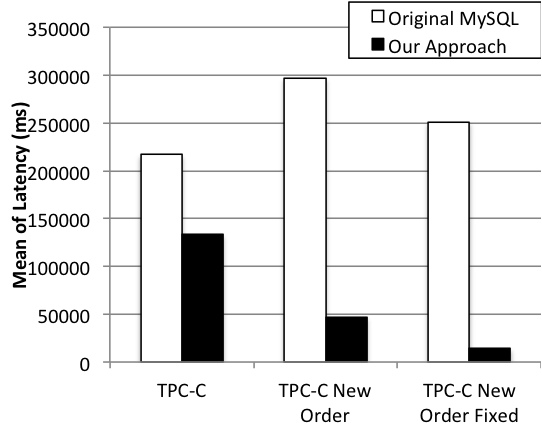
\includegraphics[width=\textwidth]{plots/all/latency}
        \caption{Average Latency}
        \label{fig:all-mean}
    \end{subfigure}
    \begin{subfigure}[t]{0.24\textwidth}
        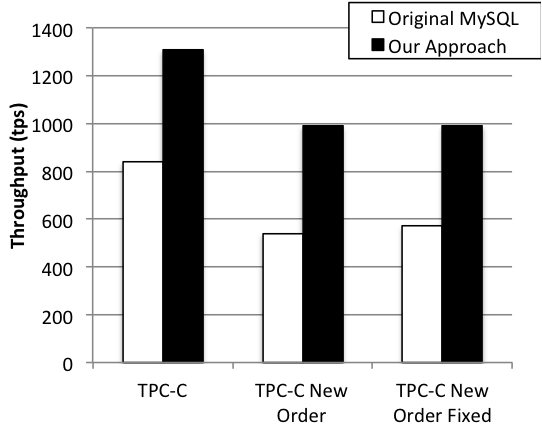
\includegraphics[width=\textwidth]{plots/all/throughput}
        \caption{Throughput}
        \label{fig:all-throughput}
    \end{subfigure}
    \begin{subfigure}[t]{0.24\textwidth}
        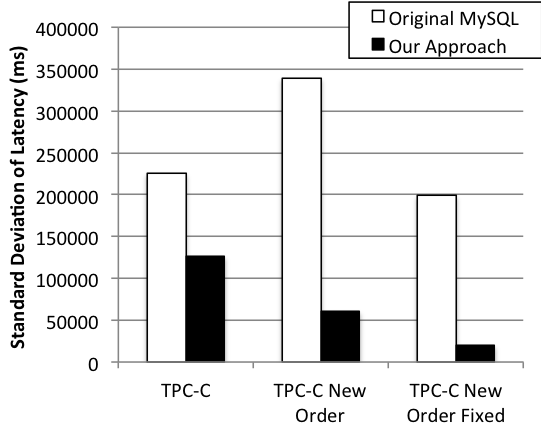
\includegraphics[width=\textwidth]{plots/all/std}
        \caption{Standard Deviation / Mean}
        \label{fig:all-std-mean}
    \end{subfigure}
    \begin{subfigure}[t]{0.24\textwidth}
        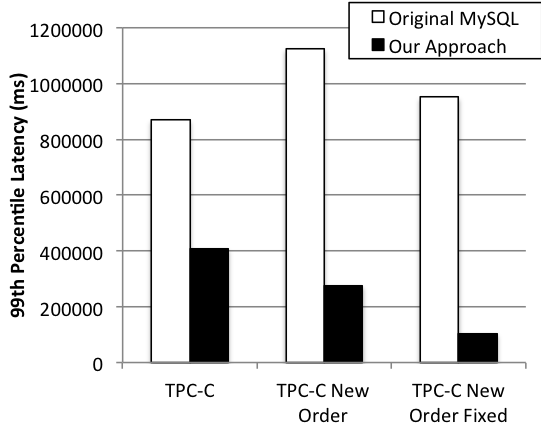
\includegraphics[width=\textwidth]{plots/all/99}
        \caption{99th Percentile / Mean}
        \label{fig:all-99-mean}
    \end{subfigure}
    \caption{Effect of All Methods Combined}
    \label{fig:all-combined}
\end{figure*}

\subsection{Evaluation of Fixes for \texttt{buf\_pool\_mutex\_enter}}
In this section we evaluate the effects of the two techniques presented in
section 5 on the variance of latency. We first implement these two techniques
in MySQL separately and run experiments on them using all three different
types of workloads. We compare the results of applying these two methods to
the original MySQL, respectively. The finer-grained locking mechanism is
referred to as ``FG'' in figure \ref{fig:fixes} and the spin lock with timeout
technique is referred to as ``SL'' in it. Both of them show improvement in
variance of latency without negative impact on the performance. Actually, they
improves not only variance, but also performance, especially the average
latency. The throughput of MySQL also receives a small increase. This is
because these two methods both reduce contention among different functions(one
by using finer-grained lock and the other by giving up lock requisition when
times out), thus reducing the time the related functions spend on waiting for
other functions. We then apply both of these two methods on MySQL, and a
greater reduction in variance than any of these two methods alone is shown.
Both standard deviation and 99th percentile reduce by more than 40\% with the
original TPC-C workload. For TPC-C New Order and TPC-C New Order Fixed, the
reductions are more than 50\%.

\begin{figure*}
    \centering
    \begin{subfigure}[t]{0.24\textwidth}
        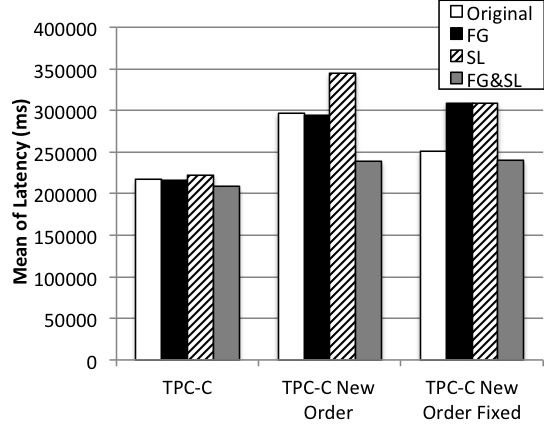
\includegraphics[width=\textwidth]{plots/ours/latency}
        \caption{Average Latency}
        \label{fig:fix-mean}
    \end{subfigure}
    \begin{subfigure}[t]{0.24\textwidth}
        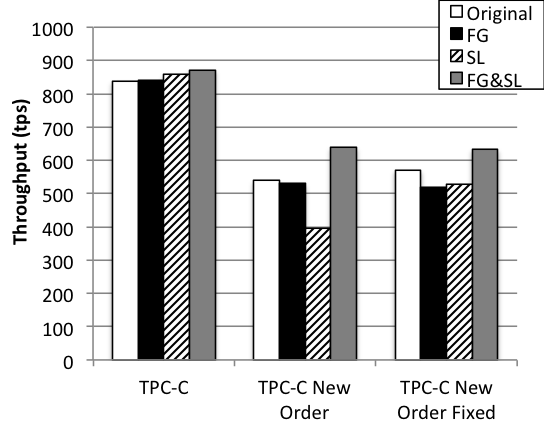
\includegraphics[width=\textwidth]{plots/ours/throughput}
        \caption{Throughput}
        \label{fig:fix-throughput}
    \end{subfigure}
    \begin{subfigure}[t]{0.24\textwidth}
        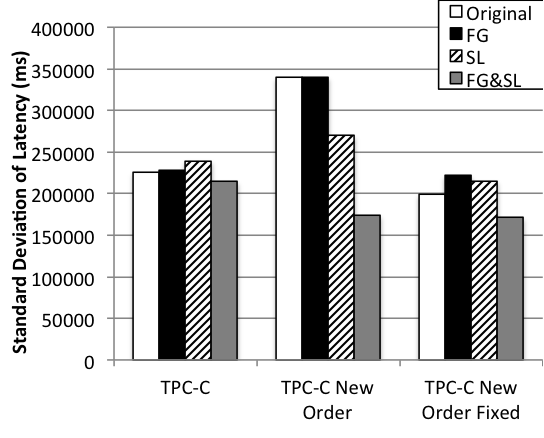
\includegraphics[width=\textwidth]{plots/ours/std}
        \caption{Standard Deviation}
        \label{fig:fix-std-mean}
    \end{subfigure}
    \begin{subfigure}[t]{0.24\textwidth}
        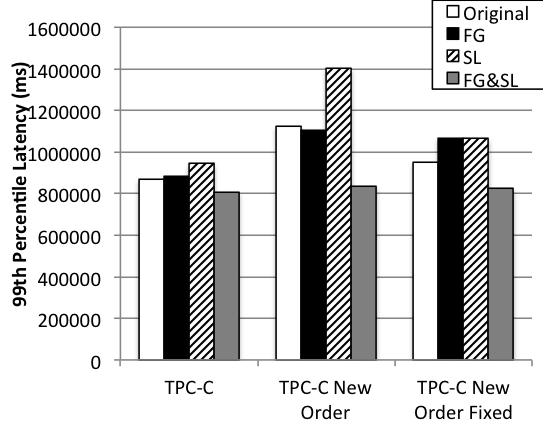
\includegraphics[width=\textwidth]{plots/ours/99}
        \caption{99th Percentile}
        \label{fig:fix-99-mean}
    \end{subfigure}
    \caption{Effect of Fixes for \texttt{buf\_pool\_mutex\_enter}}
    \label{fig:fixes}
\end{figure*}

\subsection{Using Faster Storage}
In this section we evaluate the effect of using faster storage devices on
the variance of transaction latency. We run MySQL on three different instances,
one with traditional HDD, one with SSD and one with a magnetic disk and a
ramdisk, where MySQL is installed and all the data are stored. A ramdisk is
simply a block of memory treated as a normal disk device by applications. It's
a way of simulating a super-fast disk using memory, and the data would still
be lost when powered off just like normal memory. As can be seen from figure
\ref{fig:storage}, there's huge improvement in performance when changing from
HDD to SSD and ramdisk. Also, along with that, the standard deviation and 99th
percentile of latency also decrease.

\begin{figure*}
    \centering
    \begin{subfigure}[t]{0.24\textwidth}
        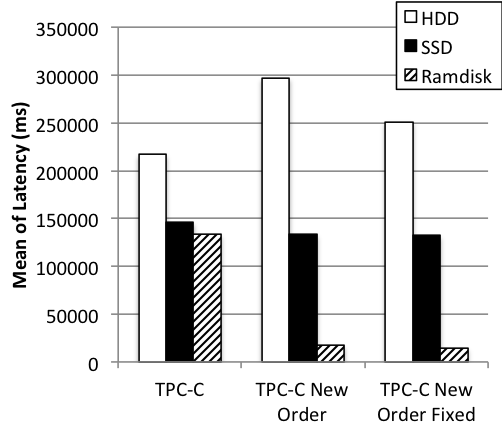
\includegraphics[width=\textwidth]{plots/storage/latency}
        \caption{Average Latency}
        \label{fig:storage-mean}
    \end{subfigure}
    \begin{subfigure}[t]{0.24\textwidth}
        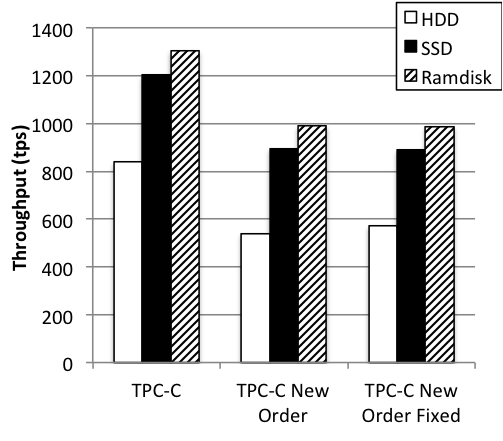
\includegraphics[width=\textwidth]{plots/storage/throughput}
        \caption{Throughput}
        \label{fig:storage-throughput}
    \end{subfigure}
    \begin{subfigure}[t]{0.24\textwidth}
        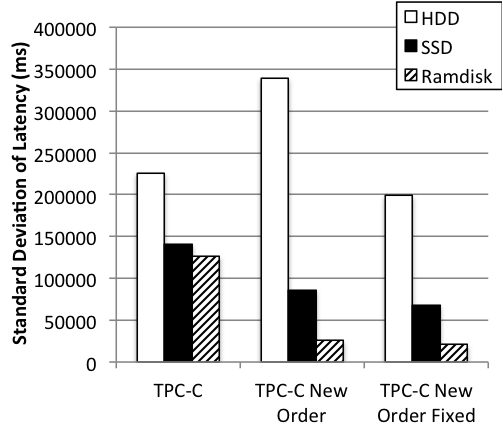
\includegraphics[width=\textwidth]{plots/storage/std}
        \caption{Standard Deviation/Mean}
        \label{fig:storage-std-mean}
    \end{subfigure}
    \begin{subfigure}[t]{0.24\textwidth}
        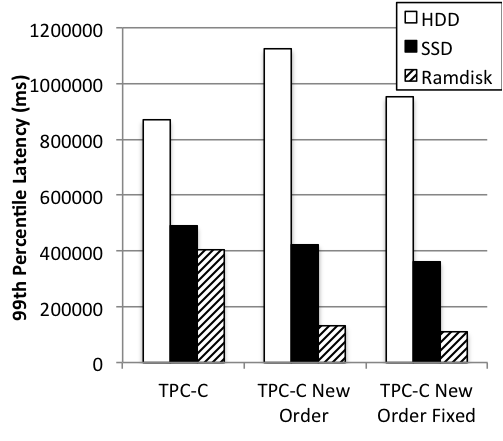
\includegraphics[width=\textwidth]{plots/storage/99}
        \caption{99th Percentile/Mean}
        \label{fig:storage-99-mean}
    \end{subfigure}
\caption{Effect of Faster Storage Device}
\label{fig:storage}
\end{figure*}

\subsection{Variance-away Tuning}
In this section, we evaluate the effects different parameters of MySQL have
on the variance of latency. We pick two parameters that we consider as
closely related to the variance of latency. The first one is the size of the
buffer pool. We increase the size of the buffer pool from 1GiB(default value)
to 5GiB. Obviously increasing the buffer pool size keeps more data in memory,
thus effectively reducing the number of buffer page replacements, the number of
I/O operations and also contention within the buffer pool. As we can see from
the results shown in figure \ref{fig:buffer_pool_size}, the larger the size of
buffer pool, the lower the average latency, standard deviation and 99th
percentile. Setting the size of the buffer pool to as large as possible is
recommended both for better performance and for higher predictability.

The second parameter that we choose and run experiments on is
\texttt{innodb\_flush\_log\_at\_trx\_commit}. This parameter affects MySQL's
strategy for flushing redo logs to disk when transactions are committed. The
default value of this option is 1, which means that logs are flushed to disk
whenever a transaction is committed. When this value is set to 0, MySQL write
the redo logs to the log files and flush the data to disk once per second, but
nothing is done when transactions commit. When this value is set to 2, redo
logs are written to the log file at transaction commit, but flush operations
are done once per second. Although this parameter is only directly related to
redo logs, changing it to 0 or 2 effectively reduces the number of I/O
operations for redo logs by grouping multiple operations into one. Experiment
result in figure \ref{fig:log_flush} shows that setting it to 0, namely
grouping multiple write operations and flush operations together, is generally
better than 2, which is to group only flush operations on performance and
variance of latency.

However, setting this option to 0 or 2 is risky. If the option is set to 0,
which means that log data is written to file and flushed to disk once per
second, and MySQL crashes, all the transactions in the last second will be gone
and cannot be recovered. On the other hand, when this option is set to 2,
namely only write the logs to the file, the transactions in the last second
will be lost when the operating system crashes(log data is safe even if MySQL
crashes with this option). Therefore, this option is only suitable for
applications that do not require high data consistency, such as forums, blogs,
but not acceptable for applications like bank systems.

\begin{figure*}
    \centering
    \begin{subfigure}[t]{0.24\textwidth}
        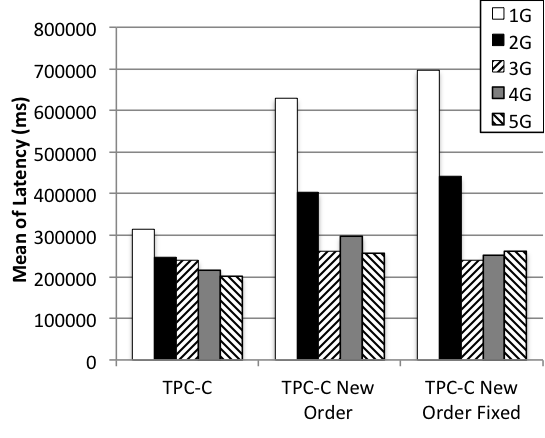
\includegraphics[width=\textwidth]{plots/buffer_pool_size/latency}
        \caption{Average Latency}
        \label{fig:buf-size-mean}
    \end{subfigure}
    \begin{subfigure}[t]{0.24\textwidth}
        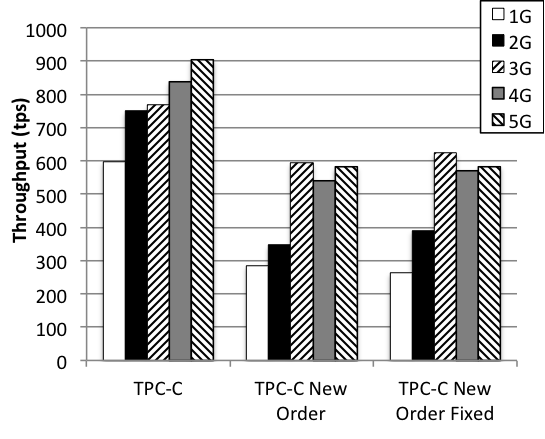
\includegraphics[width=\textwidth]{plots/buffer_pool_size/throughput}
        \caption{Throughput}
        \label{fig:buf-size-throughput}
    \end{subfigure}
    \begin{subfigure}[t]{0.24\textwidth}
        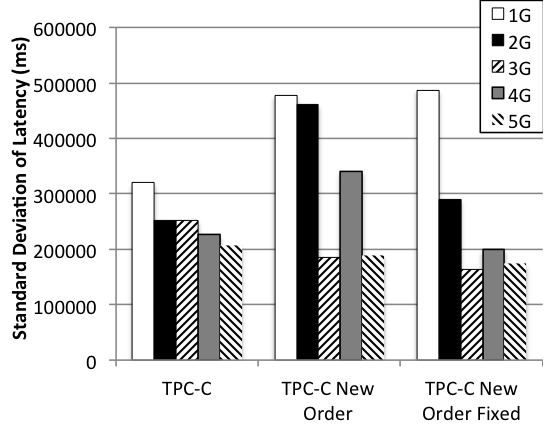
\includegraphics[width=\textwidth]{plots/buffer_pool_size/std}
        \caption{Standard Deviation}
        \label{fig:buf-size-std-mean}
    \end{subfigure}
    \begin{subfigure}[t]{0.24\textwidth}
        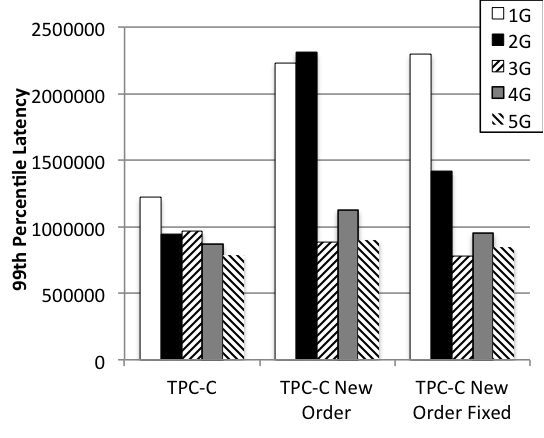
\includegraphics[width=\textwidth]{plots/buffer_pool_size/99}
        \caption{99th Percentile}
        \label{fig:buf-size-99-mean}
    \end{subfigure}
\caption{Effect of Buffer Pool Size}
\label{fig:buffer_pool_size}
\end{figure*}

\begin{figure*}
    \centering
    \begin{subfigure}[t]{0.24\textwidth}
        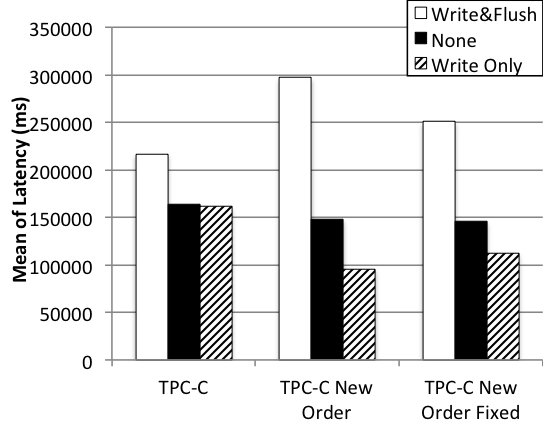
\includegraphics[width=\textwidth]{plots/log_flush/latency}
        \caption{Average Latency}
        \label{fig:commit-mean}
    \end{subfigure}
    \begin{subfigure}[t]{0.24\textwidth}
        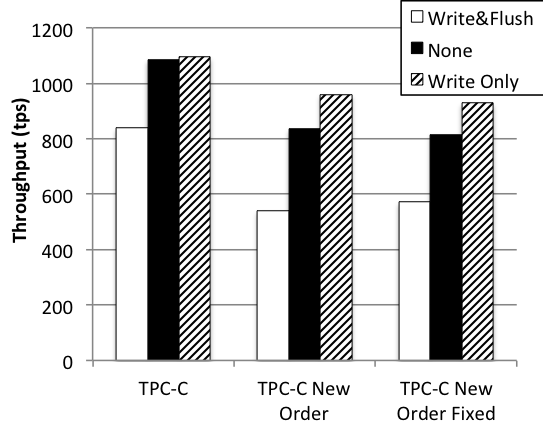
\includegraphics[width=\textwidth]{plots/log_flush/throughput}
        \caption{Throughput}
        \label{fig:commit-throughput}
    \end{subfigure}
    \begin{subfigure}[t]{0.24\textwidth}
        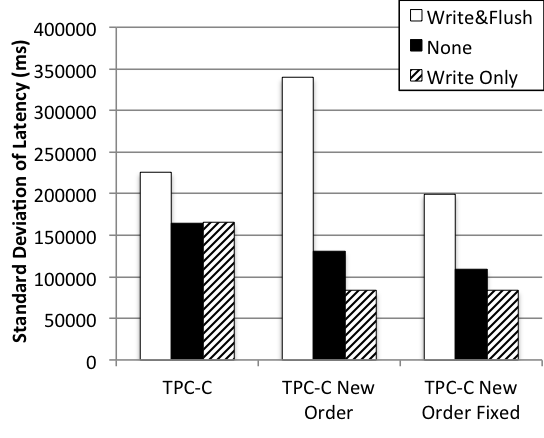
\includegraphics[width=\textwidth]{plots/log_flush/std}
        \caption{Standard Deviation}
        \label{fig:commit-std-mean}
    \end{subfigure}
    \begin{subfigure}[t]{0.24\textwidth}
        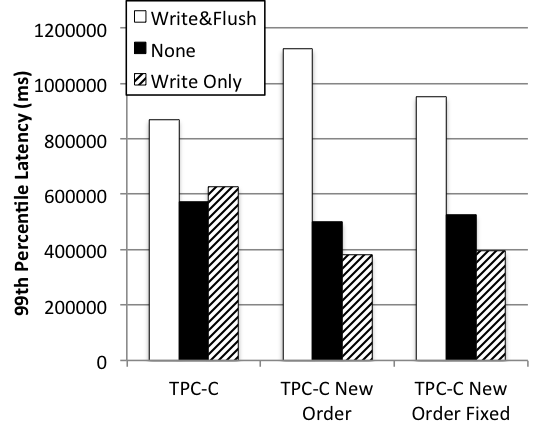
\includegraphics[width=\textwidth]{plots/log_flush/99}
        \caption{99th Percentile}
        \label{fig:commit-99-mean}
    \end{subfigure}
\caption{Effect of Log Flush Policy}
\label{fig:log_flush}
\end{figure*}

\subsection{Evaluation of VProfiler}
In this section, we evaluate the performance overhead VProfiler introduces
into MySQL when it monitors the execution time of a \textit{parent function}
and its \textit{child functions} to break down the \textit{parent function's}
variance, and its efficiency in finding the main sources of variance in MySQL.

\subsubsection{VProfiler vs. DTrace}
VProfiler breaks down the variance of a \textit{parent function} into the
variances and covariances of its \textit{child functions} by monitoring the
execution time of the \textit{parent functions} and every \textit{child
function}. This introduces overhead to the system. In this section, we change
the number of \textit{child functions} VProfile needs to monitor and measure
its performance overhead in terms of reduction average latency and throughput.

As a comparison, we also evaluate the performance overhead of DTrace. Due to
its incomplete support on Linux, we had to run a virtual machine on VirtualBox
with 10 Intel Xeon E5-2450 2.10GHz virtual CPUs and 15GiB of memory and
run Solaris 11 on it.

\begin{figure}
    \centering
    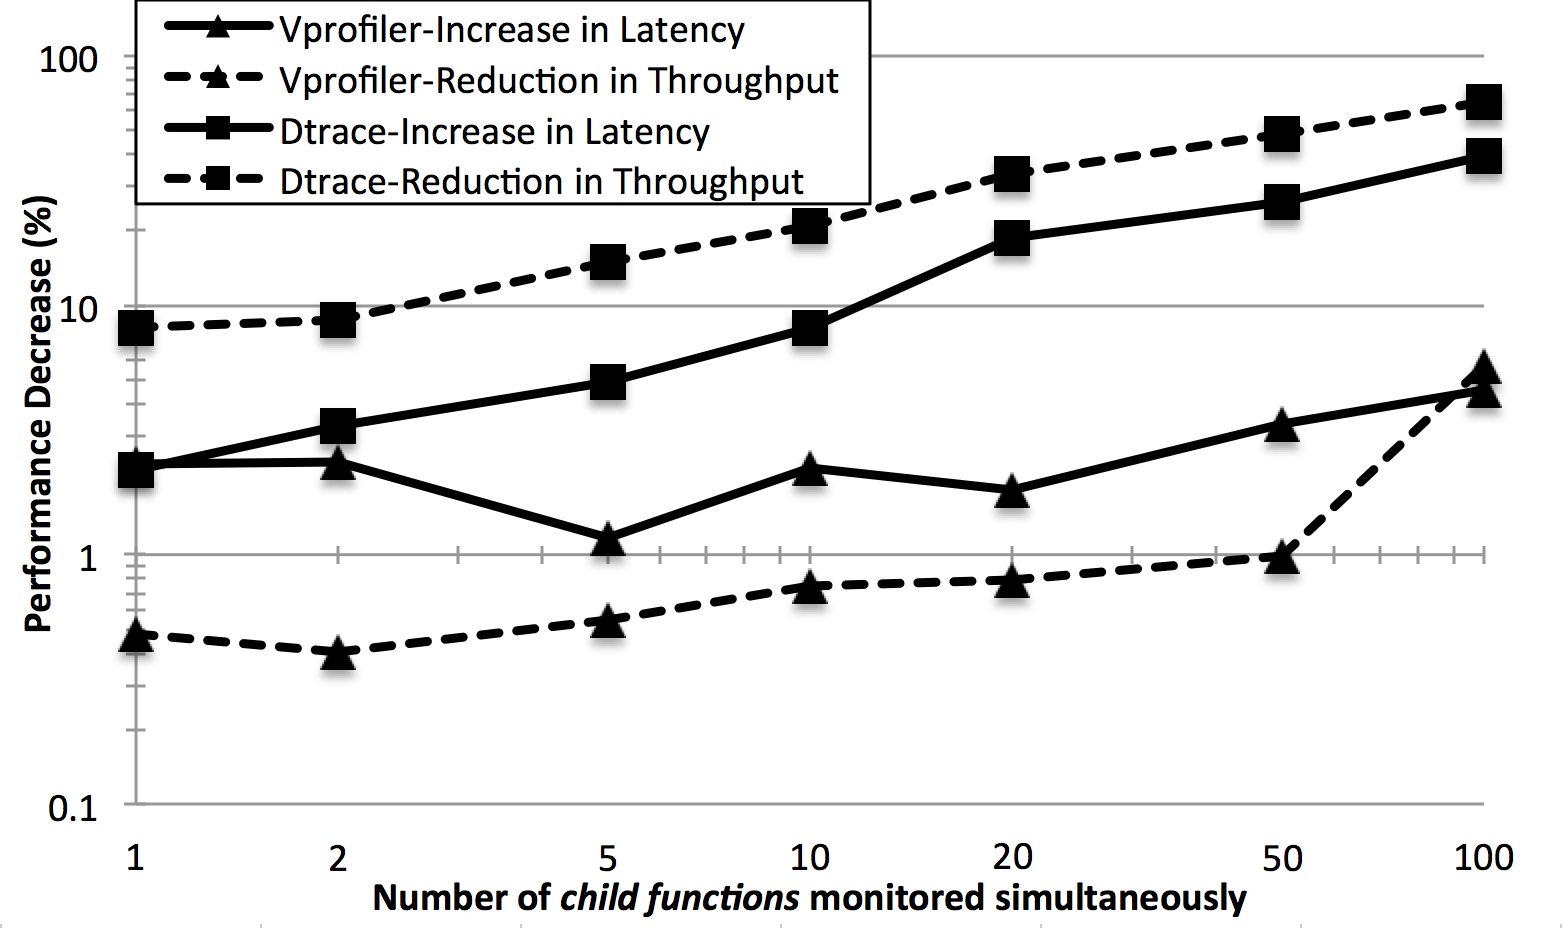
\includegraphics[scale=0.3]{plots/overhead}
\caption{Profiler overhead: VProfiler vs. DTrace}
\label{fig:overhead}
\end{figure}

In this experiment, we change the number of \textit{child functions} to trace
from 1 to 100. Figure \ref{fig:overhead} shows the experiment results. We can
see that the overhead of DTrace is a lot higher than VProfiler. The overhead of
DTrace in terms of reduction in latency and throughput grows rapidly as the
number of child functions it traces simultaneously increase, while the overhead
of VProfiler stays below 6\%, because the monitoring technique VProfiler uses
is pretty lightweight.

\subsubsection{VProfiler vs. Naïve Profiler}
In this section, we compare VProfiler to a na\"{\i}ve profiler, which is very
similar to VProfiler but breaks down every factor when possible instead of only
a few important ones. We use this profiler on MySQL and evaluate the number of
experiments this profiler has to run to find out the main sources of variance
with different numbers of functions to monitor simultaneously in each 
experiment.

\begin{figure}
    \centering
    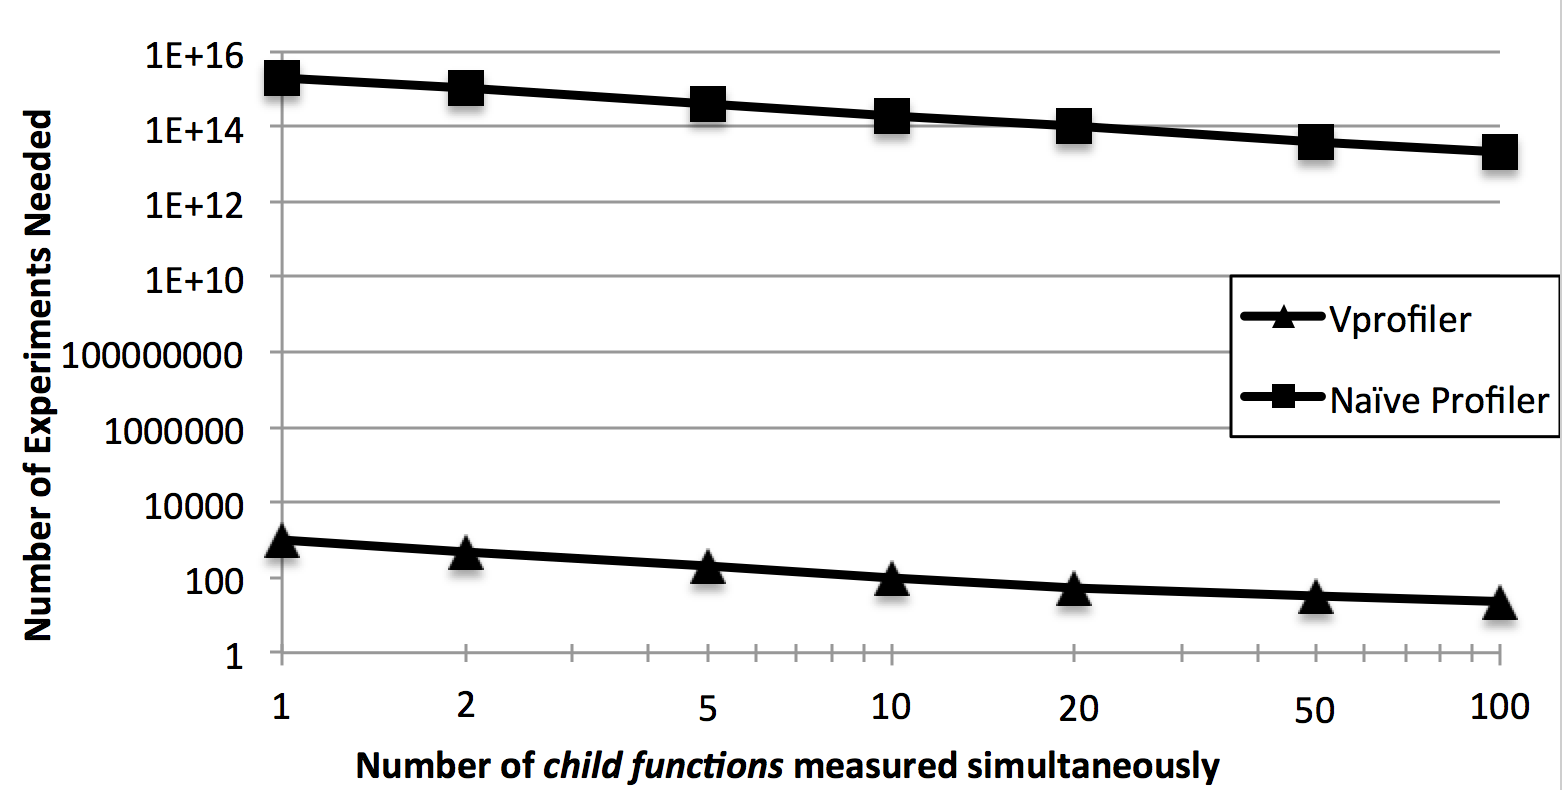
\includegraphics[scale=0.3]{plots/experiments}
\caption{Number of experiments needed for the profiler to find out the main sources of variance}
\label{fig:experiments}
\end{figure}

There are totally $2 \times 10^{15}$ nodes in the call graph(one function 
called in multiple places are regarded as different nodes in the graph),
$4.5 \times 10^{14}$ of which being leaves. Since the na\"{\i}ve profiler has
to break down every non-leaf nodes, the number of experiments needed is
extremely large. The selection strategy of VProfiler greatly reduces the number
of experiment it has to run to locate the main sources of variance.


%!TEX root = predictability.tex

\section{Conclusion}
\label{sec:conclusion}




\bibliographystyle{plain}
\bibliography{predictability}
\end{document}
